\chapter{Einführung}
\label{introduction}
%- Hintergrund
%- Motivation
%- Ziele
%- Aufgaben
%- Allgemeine Beschreibung des Projektes
%- Worum geht es in dieser Arbeit?
%- Wer hat die Arbeit veranlasst und wozu?
%- Wer soll von den Ergebnissen profitieren?
%- Welches Problem soll gelöst werden? Warum?
%- Unter welchen Umständen braucht man eine Verbesserung?
%- Was ist der Stand der Technik?
%- Welche noch offenen Probleme gibt es?
%- Worin unterscheidet sich mein Ansatz von den bisherigen?
%- Welche Ziele hat die Arbeit?
%- Wie will ich diese Ziele erreichen?
%- Was habe ich im Einzelnen vor?

Die gegenwärtig stark einhergehende Digitalisierung des privaten, beruflichen und öffentlichen Lebens verändert die Art wie Unternehmen untereinander konkurrieren, Werte schaffen und mit ihren Geschäftspartnern und Kunden interagieren \cite[S. 1]{oswald_digitale_2018}.

Die sogenannte Digitale Transformation wird ein zunehmend wichtig werdender Veränderungsprozess, um die gegenwärtigen Potenziale neuer Innovationen wie Big Data, künstliche Intelligenz oder Cloud Computing konsequent auszunutzen und stetig Wettbewerbsvorteile zu generieren \cite[S. 2]{oswald_digitale_2018}. Klassische Führungskonzepte greifen nicht mehr, Stichworte wie Flexibilität, Schnelligkeit, Dynamik und Kundenorientierung sind essentielle Voraussetzungen. 

Das Aufbrechen alteingesessener Strukturen bis hin zur Transformation zu einem digitalen Unternehmen bringt jedoch hohe Probleme mit sich. Bei einer erfolgreichen Umsetzung des Veränderungsprozesses spielen eine große Reihe von Einflüssen mit ein. Oft bremsen gerade alte Strukturen den Erfolg der Veränderungen, was gerade bei der Forderung nach Flexibilität und Dynamik ein großes Problem darstellt. \cite[S. 196]{appelfeller_digitale_2018} 

Sogenannte agile Methoden können helfen, Probleme des klassischen Change Management in der Digitalen Transformation zu bearbeiten. Praktiken wie z.B. Design-Thinking oder DevOps haben sich bereits als Projektmanagement-Instrumente bewährt \cite[S. 7]{deeken_agiles_2018}. Interessant ist jedoch auch die Herangehensweise, sie im Kontext größerer Organisationen einzusetzen, um mithilfe der Bildung einer agilen Kultur den Transformationsprozess zu optimieren \cite[S. 140]{hofert_agiler_2016}.

Im Folgenden soll auf den genauen Forschungsschwerpunkt der vorliegenden Arbeit eingegangen werden. Es wird eine Einführung über Problematiken innerhalb der Digitalen Transformation gegeben und die exakte Zielstellung der Arbeit aufgeführt. Außerdem wird nachfolgend der Aufbau der Arbeit geklärt und erläutert, mithilfe welcher Methodik die aufgeführten Fragestellungen beantwortet werden sollen.

\section{Problemstellung}

''Die Diskussion rund um digitale Transformation ist geprägt von Hypes und dringenden Warnungen, die zum Handeln anregen sollen'' \cite[S. 12]{berghaus_2016}. Innerhalb der Digitalisierung kommt es zu einem zunehmenden Druck bei der Aufrechterhaltung eines konkurrenzfähigen Geschäftsmodells. Das Aufkommen immer neuer Innovationen in verschiedenen Technologien bildet zudem eine Gefährdung, durch neue Möglichkeiten von Markteintritten, bis hin zur Zerschlagung altbewährter Geschäftsmodelle, sogenannte Digitalen Disruptionen \cite{urbach_digitalization_2018}.

Diese Gefährdungen treiben Großunternehmen dazu, gegenwärtige Strukturen zu überdenken und Veränderungen einzuleiten. Vornehmlich die Digitalisierung des Geschäftsmodells, aber auch der gesamten Unternehmensstruktur samt - kultur sind wichtige Themen in den Führungsebenen großer, internationaler Unternehmen \cite[S. 18]{buhse_transformationswerk_2016}. Das Bestreben nach Veränderungen hin zu einem digitalen Unternehmen ist also erkennbar in den Köpfen von Management und Führung. Trotzdem lassen Studien wie von \citeA{buhse_transformationswerk_2016} erkennen, dass so ein großangelegter Veränderungsprozess wie die Digitale Transformation ebenso große Problemfelder mit sich bringen kann. Oft mangelt es schon an einem erfolgreichen Wissensaustausch innerhalb des Unternehmens, beispielsweise hervorgerufen durch ''existente Vernetzungslücken und Defizite in der internen Kommunikation'' \cite[S. 18]{buhse_transformationswerk_2016}.

Zur Bekämpfung klassischer Probleme in großen Veränderungsprozessen bedarf es oft externer Hilfe. Promotoren oder Inkubatoren können helfen, Problemfelder im Transformationsprozess anzugehen. \citeA{zillmann_status_2017} geht in seiner Studie sogar soweit, dass ''$\lbrack$o$\rbrack$hne externe Beratungs- und IT-Dienstleister $\lbrack$...$\rbrack$ all diese Herausforderungen nicht zu bewältigen'' (S. 16) wären. Interne Treiber können aber ebenfalls dazu beitragen, solche Problemfelder anzugehen. Oft fehlt es allein schon an kulturellen Veränderungen innerhalb des Unternehmens. Ein sogenanntes \textit{Agiles Mindset} kann helfen, einen  solchen Kulturwandel einzuleiten. \cite{hofert_agile_2018}

Eine wesentliche Fragestellung der vorliegenden Arbeit soll sein, eine Reihe solcher Problemfeldern, die eine angestrebte Digitale Transformation gefährden, zu identifizieren. Daraus resultierend soll untersucht werden, inwieweit diese durch den Einsatz sogenannter Agiler Praktiken bzw. Methoden gelöst werden können.

\section{Forschungsfragen und Zielstellung}
\label{introduction:fs}

Die nachfolgenden Untersuchungen sollen sich mit folgenden grundlegenden
Fragestellungen beschäftigen:

\begin{itemize}[noitemsep, topsep=0pt]
	\item \textit{FS1}: Wie sehen allgemeine Veränderungsprozesse im Zuge der Digitalen Transformation aus?
	\item \textit{FS2}: Welche Probleme treten bei der Digitalen Transformation eines Groß-unternehmens auf?
	\item \textit{FS3}: Welche agilen Praktiken bzw. Methoden haben sich in großen Organisationen innerhalb des Transformationsprozesses etabliert?
	\item \textit{FS4}: Wie können agile Praktiken bzw. Methoden dazu beitragen, die vorher erarbeiteten Probleme zu beheben?
	\item \textit{FS5}: Welche Handlungsmuster lassen sich für einen erfolgreichen Einsatz agiler Praktiken bzw. Methoden im Transformationsprozess ableiten (Best Practices)?
\end{itemize}
Der erste Schwerpunkt besteht in der Extraktion verschiedener Veränderungsmuster innerhalb des Transformationsprozesses von Großunternehmen (vgl. FS1). Dies sind bestimmte Komponenten, die von der Digitalen Transformation direkt betroffen sind. Das können beispielsweise unternehmensinterne Strukturen, aber auch das Geschäftsmodell des Unternehmens sein. Grundsätzlich sollen folgende Fragen beantwortet werden: Was \textit{verändert} sich im Unternehmen? Was soll genau \textit{digitalisiert} werden? Anschließend soll weiterhin erschlossen werden,  in welchen Bereichen es vermehrt zu Problemen im Veränderungsprozess kommen kann (vgl. FS2).

Der zweite große inhaltliche Schwerpunkt ist der Einsatz agiler Praktiken im Transformationsprozess. Es werden Praktiken untersucht, die derzeit in der Digitalen Transformation weite Anwendung finden (vgl. FS3). Es soll somit eine Art \textit{Status Quo} geschaffen werden, um die Relevanz agiler Praktiken besser einschätzen zu können. Anschließend soll eine Bewertung eben dieser agilen Methoden vorgenommen werden (vgl. FS4). Als Ergebnis dessen soll die vorliegende Arbeit mögliche Best Practices für den Einsatz agiler Praktiken im Transformationsprozess erarbeiten (vgl. FS5). Dadurch kann ein Anreiz geschaffen werden, entsprechende Methoden gezielt im Veränderungsmanagement einzusetzen. 

Die konkrete Zielstellung besteht darin, agile Praktiken hinsichtlich ihrer Anwendbarkeit bei Problemen innerhalb des Digitalen Transformation von Groß-unternehmen zu evaluieren. Der genaue Aufbau dieses Vorhabens wird in den folgenden Abschnitten beschrieben.

\section{Aufbau der Arbeit}
\label{introduction:schema}

Zur Orientierung der Vorgehensweise wird ein kurzer Überblick über den Aufbau gegeben.  \ref{fig:aufbau} skizziert das wesentliche Schema der vorliegenden Arbeit.

\begin{figure}
	\centering
	\fbox{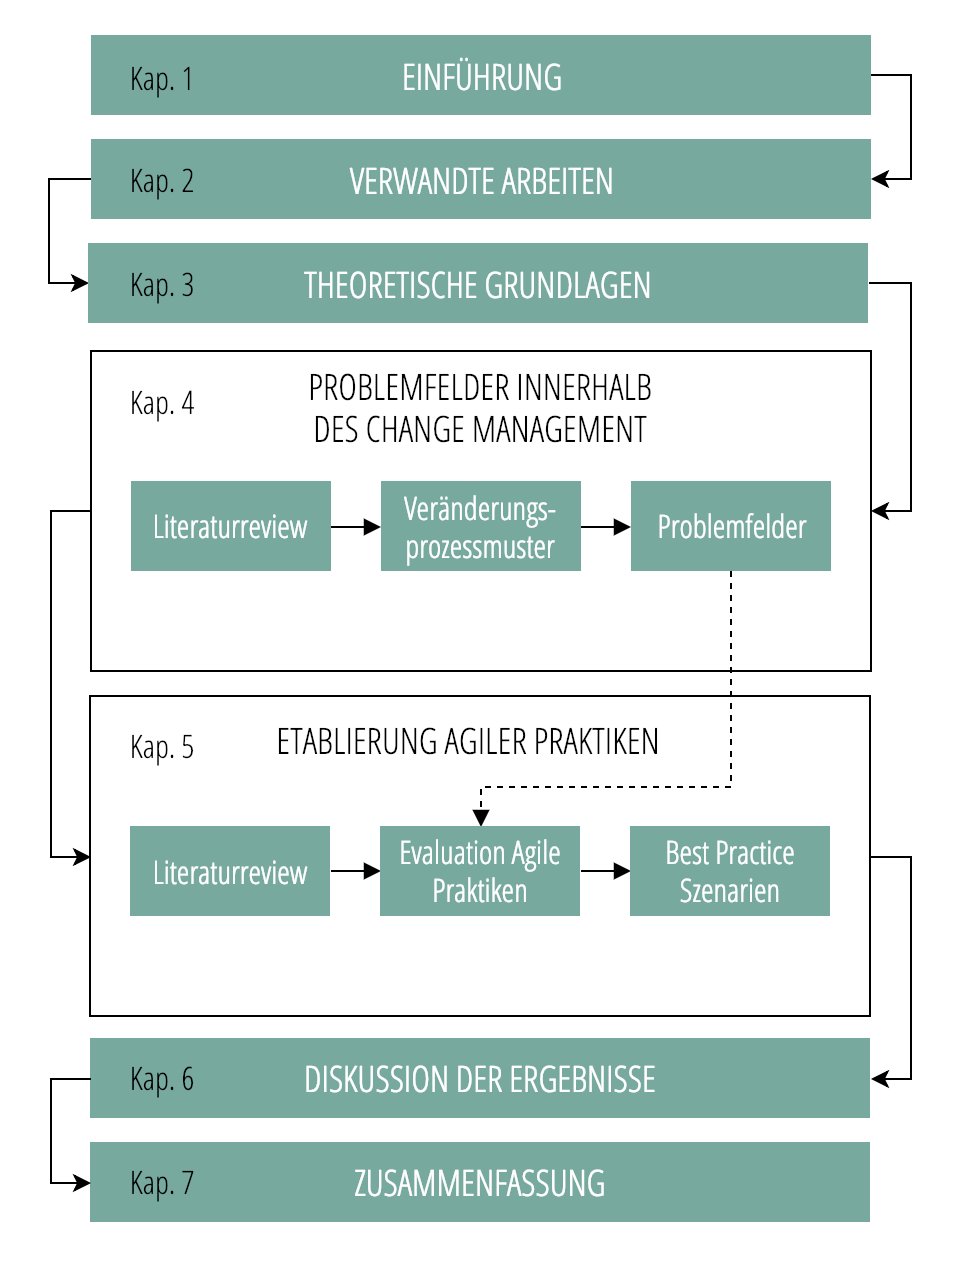
\includegraphics[width=0.5\linewidth]{pics/aufbau}}
	\caption[Aufbauschema der Arbeit]{Aufbauschema der Arbeit (eigene Darstellung)}
	\label{fig:aufbau}
\end{figure}

Aufbauend auf die Einführung in die wesentliche Problematik  (vgl. \ref{introduction}) wird anschließend ein Überblick über artverwandte Arbeiten in dem Thema aufgeführt (vgl. \ref{relatedwork}, ab S. \pageref{relatedwork}). Es wird erläutert, welcher Forschungsstand im wesentlichen bereits vorliegt und wie sich die vorliegende Arbeit abgrenzt. Zum Aufbau eines besseren Verständnisses innerhalb der Thematik schließt der einleitende Teil mit einer theoretischen Einführung in wichtige Komponenten (vgl. \ref{background}, ab S. \pageref{background}). In diesem Abschnitt werden zudem wichtige Begriffsabgrenzungen vorgenommen.

Der Hauptteil der Arbeit gliedert sich in zwei wesentliche Abschnitte. Zunächst werden in \ref{problemfields} (ab S. \pageref{problemfields}) mithilfe eines systematischen Literaturreviews relevante Veränderungsprozessmuster und Problemfelder innerhalb der Digitalen Transformation in Großunternehmen erarbeitet. Anschließend werden weiterhin durch ein zweites Literaturreview eine Reihe von genutzten agilen Praktiken bzw. Methoden im Transformationsprozess zusammengestellt, welche anschließend nach einem genauem Schema evaluiert werden (vgl. \ref{agilepractices}, ab S. \pageref{agilepractices}). Auf dieser Grundlage werden im gleichen Kapitel Best Practice Szenarien für den Einsatz agiler Praktiken im Transformationsprozess aufgestellt. Der Zusammenhang zwischen beiden Hauptteilen wird im nachfolgenden Abschnitt 1.4 erklärt.

Die Ergebnisse aus den vorhergehenden Abschnitten werden in \ref{evaluation} (ab S. \pageref{evaluation}) kritisch diskutiert. Abschließend wird eine Zusammenfassung über die Erkenntnisse der vorangestellten Untersuchungen aufgeführt (vgl. \ref{conclusion}, ab S. \pageref{conclusion}).


\section{Methodisches Vorgehen}
\label{introduction:methods}

% - allgemeines Vorgehen, mit Verweis auf die methodischen Unterkapitel der einzelnen Abschnitte. Systematischer Literaturreview + Metastudie als spezielle Form, Evaluation am Ende der zweiten Metastudie

Das übergeordnete Ziel soll die Evaluation agiler Praktiken im Kontext der Digitalen Transformation sein. Dafür soll zunächst ein systematisches Literaturreview vorgenommen werden. Dieses Review wird in zwei großen Bestandteilen durchgeführt. Zunächst soll in \ref{problemfields} (ab S. \pageref{problemfields}) eine Reihe von Fallstudien systematisch analysiert werden. Eine weiteres, methodisch vom ersten getrenntes  Review wird dann in \ref{agilepractices} (ab S. \pageref{agilepractices}) vorgenommen. Beide SLR haben das Wesen einer Metastudie, da vornehmlich Erkenntnisse vorhandener Fallstudien im Bereich der Digitalen Transformation ausgewertet und zusammengefasst werden. Allgemeine Fachliteratur wird in beiden Fällen keine große Bedeutung zuteil, mit einer  Ausnahme innerhalb des zweiten Reviews in \ref{agilepractices} (ab S. \pageref{agilepractices}). Die genaue Vorgehensweise, sowie Ein - und Ausschlusskriterien werden in den jeweiligen Abschnitten zum Methodischen Vorgehen noch erläutert (vgl. \ref{problemfields:methods}, ab S. \pageref{problemfields:methods} und \ref{agilepractices:methods}, ab S. \pageref{agilepractices:methods}).

Das Ziel der zweigeteilten Literaturreviews soll sein, relevante Ergebnisse aus bereits getätigten Studien und Fallstudien zu analysieren und zusammenzufassen, um sie für die nachfolgende Evaluation gezielt einsetzen zu können. Mithilfe der Analyse verschiedenster aktueller Studien und Fallstudien soll ein möglichst gegenwärtiges Bild der Situation in internationalen Großunternehmen dargestellt werden.

Als weiterer methodischer Schwerpunkt in der vorliegenden Arbeit wird eine Evaluation vorgenommen. Diese dient in \ref{agilepractices} (ab S. \pageref{agilepractices}) dazu, die mithilfe des Literaturreviews erarbeiteten agilen Praktiken in Bezug auf Anwendbarkeit in bestimmten Problemfeldern (vgl. \ref{problemfields}, ab S. \pageref{problemfields}) zu bewerten. Die Evaluation wird nach einem klaren Bewertungsschema vorgenommen. Das Schema und die Bewertungskriterien werden im dazugehörigen methodischen \ref{agilepractices:methods} (ab S. \pageref{agilepractices:methods}) dargestellt. Eine Diskussion zur Wahl der Methodik wird in \ref{evaluation} (ab S. \pageref{evaluation}) vorgenommen.
